% !TeX root = 00General.tex
\thispagestyle{standard}
\pagestyle{standard}
\chapter{Ausgangslage}

Im Auftrag einer Firma, die vor kurzer Zeit durch einen Netzwerkausfall erheblichen Schaden erlitten hat, soll das Firmennetzwerk ausfallsicherer gemacht werden. Eine Bedingung ist, dass keine neue Hardware angeschafft werden soll. Abbildung \ref{img:Ausgangslage} zeigt den derzeitigen Netzwerkaufbau.

\begin{figure}[H]
	\centering
	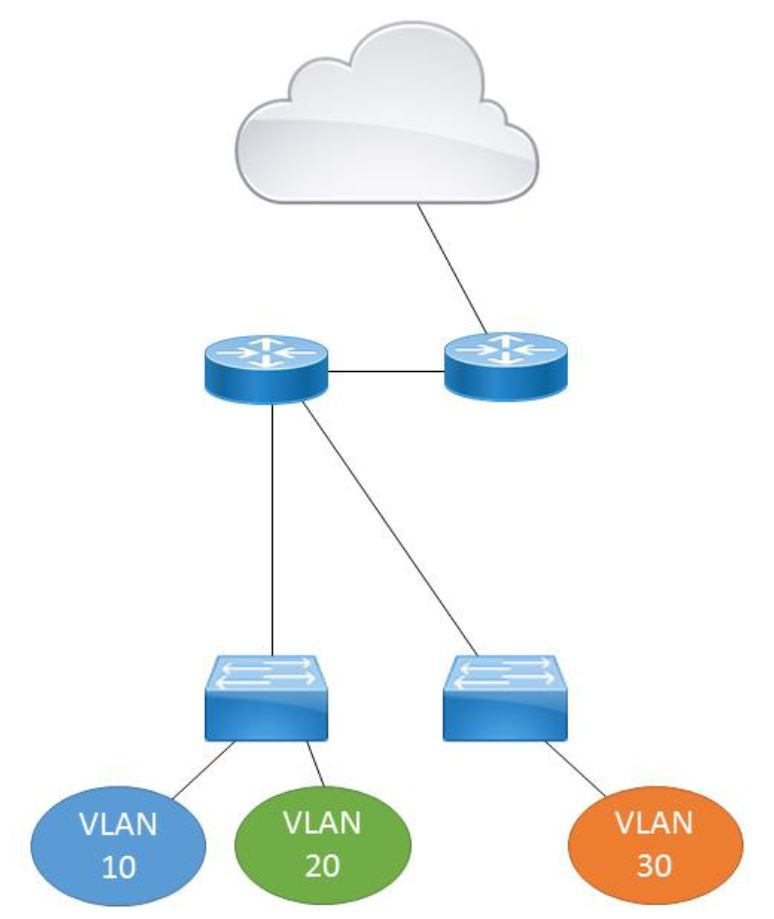
\includegraphics[width=0.9\textwidth]{img/Ausgangslage.JPG}
	\caption{Ausgangslage Netzwerktopologie}
	\label{img:Ausgangslage}
\end{figure}

\chapter{Netzwerkplanung}

Das zu planende Netzwerk soll im Hinblick auf Netzzuverlässigkeit optimiert werden. Dazu fordert der Kunde eine redundante Internetanbindung. Diese wird mit einer seriellen Verbindung zu \ac{ISP} 1, durch Punkt 1 in Abbildung \ref{img:Netzwerkplanung} dargestellt, erreicht. 

\begin{figure}[H]
	\centering
	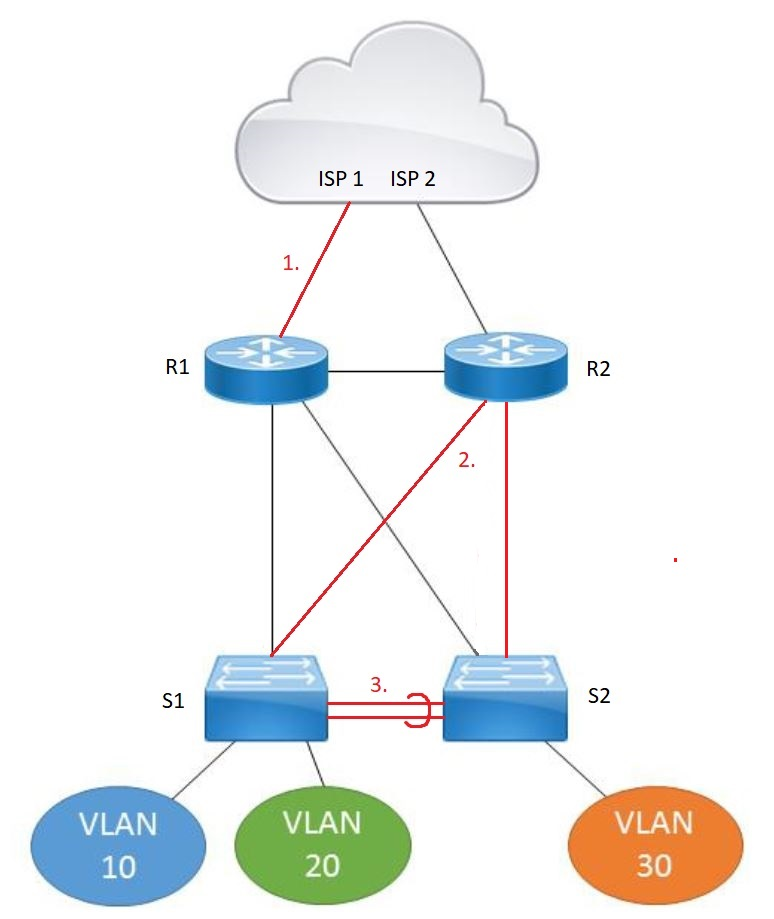
\includegraphics[width=0.9\textwidth]{img/Planung_neu.JPG}
	\caption{Planung des ausfallsicheren Netzwerks}
	\label{img:Netzwerkplanung}
\end{figure}

Durch die in Punkt 2 ergänzten Verbindungen wird eine Ausfallsicherheit für Router 1 und Router 2 erzeugt. Es wird dadurch möglich, dass im Falle eines Ausfalls von Router 1 denoch Verbindungen von \ac{VLAN} 10 in \ac{VLAN} 30 aufgebaut werden können.

Punkt 3 in Abbildung \ref{img:Netzwerkplanung} zeigt die Implementierung von EtherChannel. Werden in nächster Zeit weitere \ac{VLAN}s an verschiedene Router gehängt, so entsteht durch EtherChannel eine Bandbreitenerhöhung bzw. Load-Balancing zwischen z.B. \ac{VLAN} 10 an Switch 1 und Switch 2. Des weiteren hat EtherChannel einen sogenannten "Fail-Over Mode". Die EtherChannel Technologie verteilt die Last automatisch auf die verbleibenden Links.

\textbf{\ac{VLAN} \ac{IP} Adressen Bereich:} 

\begin{itemize}  
\item VLAN 10: 192.168.5.0/24
\item VLAN 20: 192.168.15.0/24
\item VLAN 30: 192.168.25.0/24
\end{itemize}

\chapter{Konfiguration des Netzwerks}

\section{Switches}

Um nun die EtherChannel Technologie zu realisieren wurden die Ports "FastEthernet 23 und 24" verwendet. Diese werden als sogenannte "Trunk Links" konfiguriert.

\lstset{escapeinside={\%*}{*)},numbers=left}%oder numbers=left
\begin{lstlisting}[caption={Setting EtherChannel on a switch},label={lst:etherchannel},language={}]
interface FastEthernet0/24
 switchport trunk allowed vlan 10,20,30
 switchport mode trunk
 channel-protocol lacp
 channel-group 1 mode active
\end{lstlisting}

Des weiteren wurden die verschiedenen \ac{VLAN}s, die auf den jeweiligen Switches hängen, eingestellt.

\lstset{escapeinside={\%*}{*)},numbers=left}%oder numbers=left
\begin{lstlisting}[caption={VLAN Konfiguration auf Switch 1},label={lst:vlan},language={}]
interface Vlan10
 ip address 192.168.5.254 255.255.255.0
!
interface Vlan20
 ip address 192.168.15.254 255.255.255.0

\end{lstlisting}

\section{Router}

Als internes Routing Protokoll wurde \ac{OSPF} verwendet. Um \ac{OSPF} richtig zu konfigurieren muss jedem Router eine eindeutige "router-id" zugewiesen werden, sowie alle bekannten Netze in der entsprechenden Area eingetragen werden.

\lstset{escapeinside={\%*}{*)},numbers=left}%oder numbers=left
\begin{lstlisting}[caption={OSPF Konfiguration auf Router 1},label={lst:ospf},language={}]
router ospf 10
 router-id 1.1.1.1
 network 10.10.10.0 0.0.0.255 area 0
 network 172.16.5.0 0.0.0.3 area 0
 network 192.168.5.0 0.0.0.255 area 0
 network 192.168.15.0 0.0.0.255 area 0


\end{lstlisting}